\documentclass[lang=cn,11pt,a4paper,cite=authoryear,twocolumn]{elegantpaper}

% 微分号
\newcommand{\dd}[1]{\mathrm{d}#1}
\newcommand{\pp}[1]{\partial{}#1}

\newcommand{\homep}[1]{\textbf{Problem #1}}
\newcommand{\subhomep}[1]{\textbf{SubProblem #1}}

% FT LT ZT
\newcommand{\ft}[1]{\mathscr{F}[#1]}
\newcommand{\fta}{\xrightarrow{\mathscr{F}}}
\newcommand{\lt}[1]{\mathscr{L}[#1]}
\newcommand{\lta}{\xrightarrow{\mathscr{L}}}
\newcommand{\zt}[1]{\mathscr{Z}[#1]}
\newcommand{\zta}{\xrightarrow{\mathscr{Z}}}

% 积分求和号

\newcommand{\dsum}{\displaystyle\sum}
\newcommand{\aint}{\int_{-\infty}^{+\infty}}

% 简易图片插入
\newcommand{\qfig}[3][nolabel]{
  \begin{figure}[!htb]
      \centering
      \includegraphics[width=0.4\textwidth]{#2}
      \caption{#3}
      \label{#1}
  \end{figure}
}

% 表格
\renewcommand\arraystretch{1.5}


% 日期


\title{数字电路基础\quad 第六周作业}
\author{范云潜 18373486}
\institute{微电子学院 184111 班}
\date{\zhtoday}

\begin{document}

\maketitle

作业内容:
4.3;
4.6;
4.8;4.10;
4.12;4.17
4.28;
4.32 ;

\homep{4.3}

\(Y_1 = (ABC)+(A+B+C)(AB+AC+BC)'\) 

\(Y_2 = AB + AC + BC\) 

\begin{lstlisting}
    a b c y1 y2
    0 0 0 0 0
    0 0 1 1 0
    0 1 0 1 0
    0 1 1 0 1
    1 0 0 1 0
    1 0 1 0 1
    1 1 0 0 1
    1 1 1 1 1
\end{lstlisting}

这是一个全加器,\(Y_2\) 是进位, \(Y_1\) 是加法和。

\homep{4.6}

建立真值表,但是由于水位的顺序性,不会产生特定的输入序列:

\begin{lstlisting}
    a b c ml ms 
    0 0 0 0  0
    0 0 1 0  1
    0 1 0 x  x
    0 1 1 1  0
    1 0 0 x  x
    1 0 1 x  x 
    1 1 0 x  x
    1 1 1 1  1
\end{lstlisting}

对于无关项可以任意假设,那么 \(M_L = B\) , \(M_S = A + B'C\) \footnote{也可以使用卡诺图,但是本题目较为简单。}。

\homep{4.8}

32 位信号分为 4 个字输入到 74HC148 中,若是第 i 高位未检测到,那么下一位进行检测,若是已经检测到,下一位可以不用进行检测。注意到模块在检测到 0 之后,\(Y_S' = 1\) ,因此借此进行模块之间的传输,关停后续模块。若是某个模块检测到第 n/8 位的数据,那么输出 \(\text{not } n\) 。之后模块输出 \(111, 1,1\) ,之前模块输出 \(111, 0,1\) ,可以借此进行位选,确定发生的位置,若是寻址成功则为 \(Y_{EX}' = 0 \)。对于五位的输出,高二位确定发生的字位置,低三位确定发生的比特位置。

最终如 \figref{01} 所示。

\begin{figure*}[!htb]
    \centering
    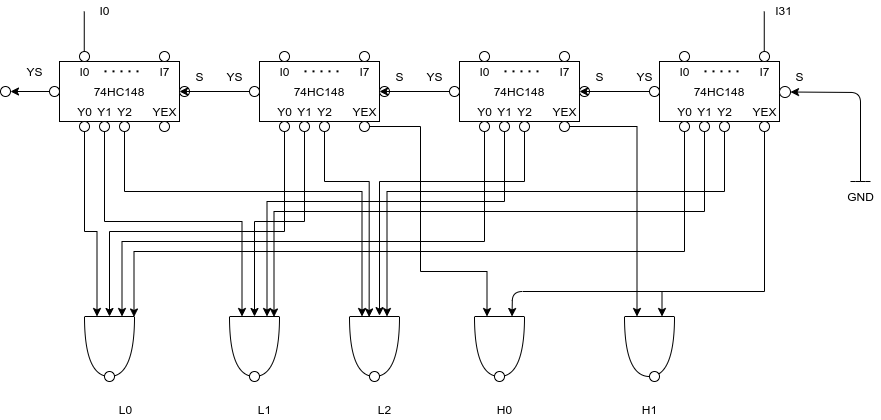
\includegraphics[width=0.8\textwidth]{hw06p1.png}
    \caption{32位解法}
    \label{01}
\end{figure*}

\homep{4.10} 

这是一个十进制译码器,

\(Z_1 = (Y_1' Y_4' Y_7')' = M'N'P'Q + M'NP'Q' + M'NPQ\)

\(Z_2 = (Y_2' Y_5' Y_8')' = M'N'PQ' + M'NP'Q + MN'P'Q'\)

\(Z_3 = (Y_3' Y_6' Y_9')' = M'N'PQ + M'NPQ' + MN'P'Q\)

\homep{4.12}

将 \(A, B, C\) 连接到 \(A_0, A_1, A_2\) ,为了使得译码器工作, \(S_1 = 1\) , \(S_2 + S_3 = 0\) 。

\(Y_1 = AC = (Y=5) | (Y=7)\)

\(Y_2 = A'B'C + AB'C' + BC = (Y=1) | (Y=4) | (Y=3) | (Y=7)\)

\(Y_3 = B'C' + ABC' = (Y=0) | (Y=4) | (Y=6)\) 

由第摩根定律和反向输出可知,需要与非门,如 \figref{02} 。

\begin{figure*}[!htb]
    \centering
    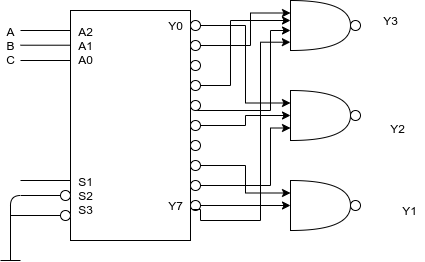
\includegraphics[width=0.8\textwidth]{hw06p2.png}
    \caption{3-8译码器}
    \label{02}
\end{figure*}

\homep{4.17}

这是两个 2 位 MUX ,但是有着相反的使能信号,一侧输出另一侧则输出 0 ,经过或门之后仍为原输出,因此可以看作一个 3 位 MUX ,将左侧的 \(D_3 - D_0\) 看作 \(D_7-D_4\) ,那么 \(Z = Q(PNM + PNM' + P'N'M + P'N'M')\) 。


\homep{4.28}

10 位比较器至少需要 3 片, 并且将高 2 位设置为相同。高位优先,若是高位比较完毕,那么低位就不必比较。

如 \figref{03} 。

\begin{figure*}[!htb]
    \centering
    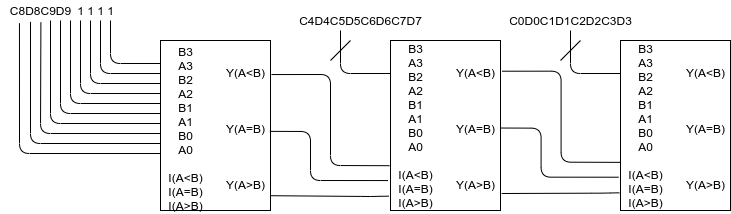
\includegraphics[width=0.8\textwidth]{hw06p3.png}
    \caption{10 位比较器}
    \label{03}
\end{figure*}



\homep{4.32}

\(Y = ((A'CD)' (AB'D)' (BC')' (CD')')' = A'CD + AB'D + BC' + CD'\)

\begin{itemize}
    \item \(A\) : \(B = 0, C = 1, D = 1\)
    \item \(B\) : \(A = 1, C = 0, D = 1\)
    \item \(C\) : \(A = 0, B = 1\) , \(A = 1, B = 1, D = 0\) 
    \item \(D\) : \(A = 0, C = 1\), \(A = 1, B = 0, C = 1\)
\end{itemize}
% Start Here

% End Here

\end{document}